\clearpage
\section{LW0 Parte 1 — Operar o Lite 6}
\textbf{Evidência:} leituras do Studio e SDK registadas pelo grupo, scripts \source{logs\_joints.py} e \source{safe\_session.py}, dados \source{juntas\_30s.csv}. A sessão segura é entregue também como código.

\subsection{Ligação e Live Control}
Na sessão documentada foi usada a rede \source{Robot-1}; o controlador tinha IP \source{192.168.1.182}, o portátil \source{192.168.1.12/24}, e o Studio foi acedido no porto \source{18333}. O primeiro erro observado foi \emph{Controller Error Code C2 — The Emergency Stop button is pushed in to Stop}. Depois de libertar a paragem, limpar o erro e ativar o braço, foi possível operar em modo de posição.

\begin{center}\small
\begin{tabular}{@{}lcc@{}}\toprule
Junta & Especificação/controlador (graus) & Extremos observados (graus)\\\midrule
J1 & $[-360,360]$ & $[-360,360]$\\
J2 & $[-150,150]$ & $[-143{,}3,148{,}6]$\\
J3 & $[-3{,}5,300]$ & $[-2{,}7,299{,}9]$\\
J4 & $[-360,360]$ & $[-360,360]$\\
J5 & $[-124,124]$ & $[-121{,}7,122{,}1]$\\
J6 & $[-360,360]$ & $[-360,360]$\\\bottomrule
\end{tabular}
\captionof{table}{Gamas da ficha e extremos ensaiados; os extremos observados não redefinem os limites.}
\end{center}

No referencial Base executaram-se X+, Y+, Z+, RX+, RY+ e RZ+, nessa ordem. A tabela transcreve as leituras de posição (mm) e orientação (graus) após cada comando; as translações avançaram 1 mm no eixo solicitado, enquanto as rotações mantiveram a posição e alteraram a orientação apresentada.
\begin{center}\small
\begin{tabular}{@{}lrrrrrr@{}}\toprule
Comando & $x$ & $y$ & $z$ & Roll & Pitch & Yaw\\\midrule
Inicial & $-2{,}6$ & $-261{,}7$ & $257{,}0$ & $174{,}5$ & $-38{,}0$ & $-29{,}7$\\
X+ & $-1{,}6$ & $-261{,}7$ & $257{,}0$ & $174{,}5$ & $-38{,}0$ & $-29{,}7$\\
Y+ & $-1{,}6$ & $-260{,}7$ & $257{,}0$ & $174{,}5$ & $-38{,}0$ & $-29{,}7$\\
Z+ & $-1{,}6$ & $-260{,}7$ & $258{,}0$ & $174{,}5$ & $-38{,}0$ & $-29{,}7$\\
RX+ & $-1{,}6$ & $-260{,}7$ & $258{,}0$ & $175{,}6$ & $-37{,}5$ & $-30{,}4$\\
RY+ & $-1{,}6$ & $-260{,}7$ & $258{,}0$ & $175{,}0$ & $-36{,}7$ & $-30{,}0$\\
RZ+ & $-1{,}6$ & $-260{,}7$ & $258{,}0$ & $175{,}0$ & $-36{,}7$ & $-29{,}0$\\\bottomrule
\end{tabular}
\captionof{table}{Leituras do Studio na sequência de comandos cartesianos.}
\end{center}
As rotações também alteraram várias juntas; estas leituras, por si só, não determinam uma convenção de Euler. O Studio indicou estado \emph{Normal}, modo \emph{Position} e montagem \emph{Floor}, com carga TCP de $0{,}28$ kg e juntas $[250{,}7,-4{,}2,49{,}0,-313{,}0,50{,}8,251{,}8]^\circ$. Com a carga definida, o braço foi guiado à mão e manteve a posição ao ser largado. A garra abriu e fechou; não foram registadas medições com paquímetro.

Durante o ensaio surgiu \emph{C22 — Self-collision Error}. No contacto com a bancada, o controlador emitiu \emph{C31 — Abnormal current in the robotic arm}, junta 2, com binário teórico de $10{,}661$ N\,m e real de $-32{,}36$ N\,m; o movimento foi interrompido. A recuperação observada foi limpar o erro, ativar, repor modo e estado. A sensibilidade de colisão registada foi 3, com carga de $0{,}277$ kg e centro de massa $[0,0,30]$ mm.

\subsection{Cinco exercícios Python}
\begin{enumerate}\setlength{\itemsep}{1pt}
\item \textbf{Leitura antes/depois do ensino:} com \source{get\_servo\_angle()} e \source{get\_position()}, as juntas passaram de $[250{,}7,-4{,}2,49{,}0,-313{,}0,50{,}8,251{,}8]^\circ$ para $[291{,}0,-4{,}2,49{,}0,-261{,}7,91{,}4,339{,}0]^\circ$. A pose passou de $[-1{,}6,-260{,}6,258{,}1,174{,}9,-36{,}7,-29{,}0]$ para $[217{,}6,-160{,}3,394{,}3,-82{,}2,15{,}2,-70{,}7]$ (mm e graus).
\item \textbf{Gamas:} os limites lidos do controlador coincidiram com a especificação da tabela acima.
\item \textbf{Home:} de três configurações iniciais, \source{set\_servo\_angle(..., speed=20, wait=True)} regressou a $[291,-4{,}2,49,-261{,}7,91{,}4,339]^\circ$. As partidas foram $[341{,}915,6{,}498,49,-254{,}400,91{,}400,339]$, $[257{,}582,-4{,}200,32{,}737,-261{,}700,91{,}400,339]$ e $[297{,}525,3{,}650,49,-248{,}089,69{,}308,316{,}976]^\circ$. Nas leituras finais impressas, a dispersão entre chegadas foi $0^\circ$ e o maior desvio absoluto foi $0{,}000020^\circ$; isto caracteriza as leituras do controlador, não a repetibilidade física independente.
\item \textbf{Cartesianas:} \source{set\_position()} aumentou Z de $394{,}182739$ para $444{,}182678$ mm ($\Delta z=49{,}999939$ mm) e regressou a $394{,}182800$ mm.
\item \textbf{Garra:} \source{open\_lite6\_gripper()}, \source{close\_lite6\_gripper()} e \source{stop\_lite6\_gripper()} foram aceites; o programa terminou com código 0.
\end{enumerate}

\subsection{Exemplos do SDK e registo temporal}
O exemplo \source{0002-get\_property} leu estado 2, modo 0, erros e avisos 0, pose e ângulos; foi adaptado o IP, sem movimento. O \source{2001-move\_joint} foi adaptado ao Lite 6: em vez das poses do xArm6, J1 avançou de $291{,}129768^\circ$ para $293{,}129792^\circ$ e voltou, com $10^\circ$/s, pausas e verificações de retorno. Assim foram exercitados \source{get\_servo\_angle()} e \source{set\_servo\_angle()} sem reutilizar limites de outro braço.

\begin{center}
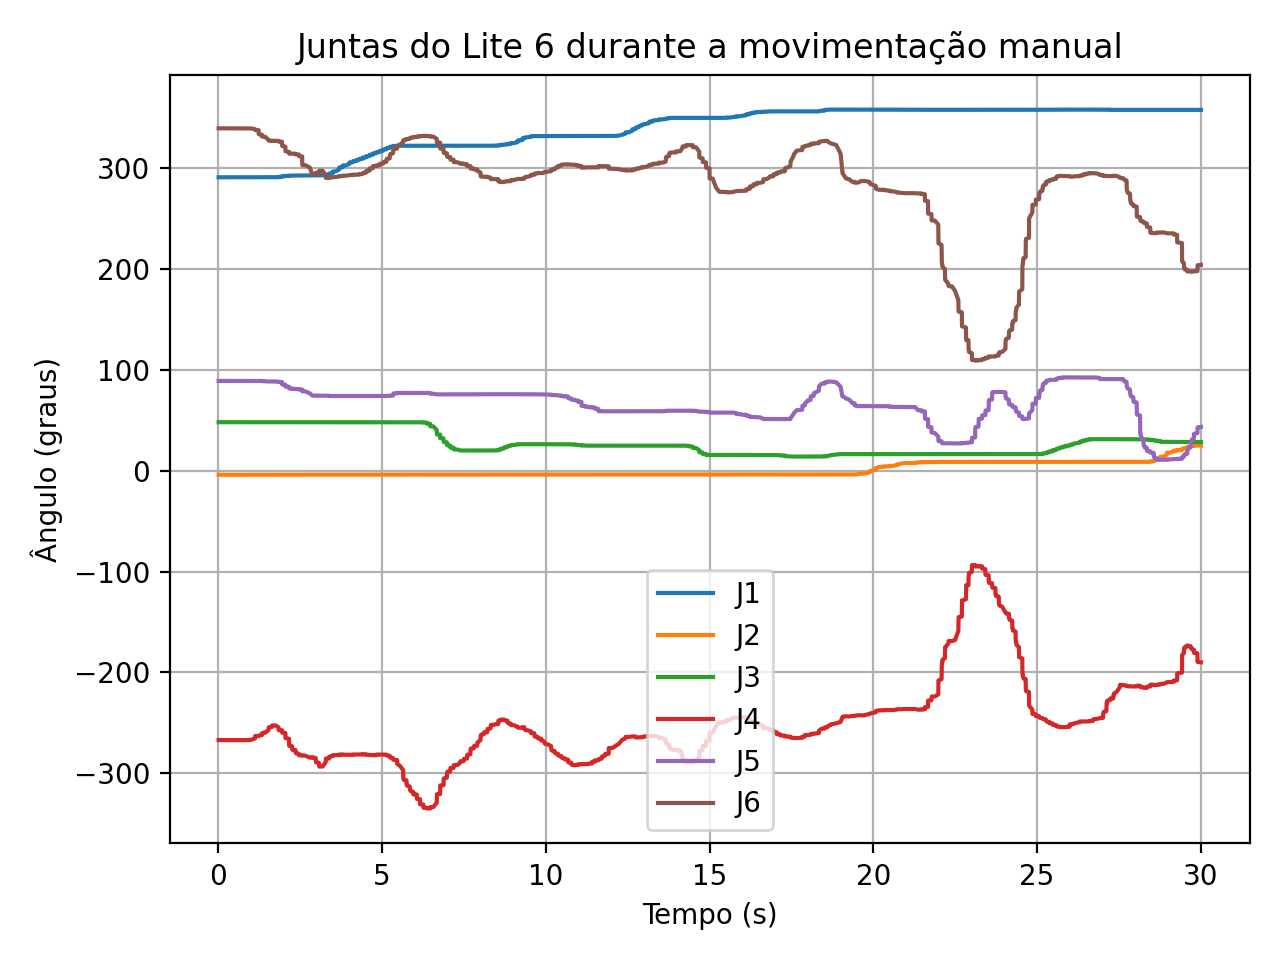
\includegraphics[width=0.78\linewidth,height=0.27\textheight,keepaspectratio]{images/lw0_juntas_30s.png}
\captionof{figure}{Ângulos das seis juntas durante orientação manual (gráfico original do grupo).}
\end{center}
O registo contém 1712 amostras em 30,00 s, sem pausa deliberada: $f_s=(N-1)/(t_{\mathrm{fim}}-t_{\mathrm{início}})=57{,}03$ amostras/s. As maiores variações visuais ocorrem em J4 e J6. A \source{safe\_session()} entregou a sessão com modo reduzido ativo, limites de $54^\circ$/s nas juntas e 150 mm/s no TCP e fronteira $[300,0,200,-200,400,10]$ mm.
